\section{Overview}

\begin{figure}[t!]
    \centering
    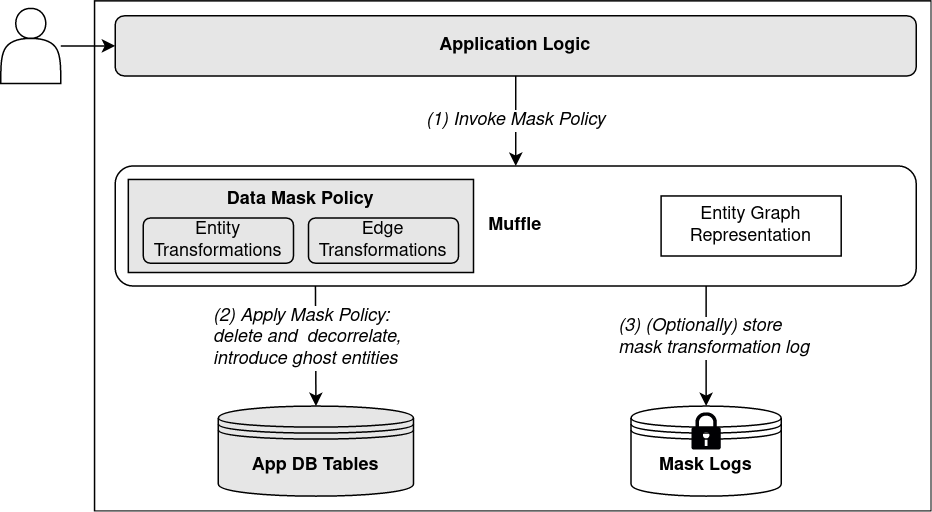
\includegraphics[width=0.5\textwidth]{img/muffle}

    \caption{High-level \sys architecture. Developers specify grayed-out components.}
    \label{fig:arch}
\end{figure}

Data masking enables developers to clearly specify data masks that can achieve a wide range of
fine-grained and expressive privacy policies. 

The key observation behind data masking is that application data naturally encodes a graph of 
entity nodes and edges, where each entity type corresponds to an application table, such as a users,
papers, or reviews table, and edges between entities are foreign key relationships. Foreign key table
columns create child-parent correlations, where the child entity is a table row that contains the parent entity's
identifier column value as a foreign key. 
%\sys also includes abstract entities in the graph, where the keys may be non-referential
%identifiers that refer to abstract, non-table entities (e.g.,\ a \texttt{thread\_id} column in the
%comments table).  

Developers specify a \emph{data mask} to specify how the privacy policy constrains the structure and
content of the entity graph (Section~\ref{sec:policies}). A mask corresponds to a piece of the
application privacy policy, \eg unsubscription, and specifies the end state of the entity graph
after a user unsubscribes. 

Developers use their application expertise to determine an acceptable post-mask state, balancing
data retention with data anonymization, decorrelation, and deletion, all while maintaining
application correctness.  Specifying post-mask state requires the developer to reason only at the
level of entity and edge \emph{types}, instead of about specific entity graph instances.
%Furthermore, the declarative mask specification also provides a precise post-mask specification for users and
%developers.
 
Masks transform the entity graph by introducing \emph{ghost entities}, which both replace real
entities and break structural correlations.  Decorrelating, modifying, and deleting entities in the
graph can expressed via transformations that produce ghost entities from real entities, and
restructure the entity graph with edges to ghost entities. 
%the application entity
%graph and how the mask transforms of this graph, and systematically applies the transformation when
%invoked (Figure~\ref{fig:arch}).

Data masking additionally supports reversible masks: developers can specify whether to save (and
potentially encrypt) the graph transformations performed by the mask, which allows future unmasking
of data to support \eg resubscription after unsubscription.

We design and implement an initial prototype, which sits between the application logic and its
database (Figure~\ref{fig:arch}). Our prototype takes a data mask as input, and systematically
applies the appropriate data transformations to ensure the resulting abstract entity graph matches
the state specified by the data mask.
